\chapter{Introduction to LLMOps and the Ishtar AI Case Study}
\label{ch:intro}
\newrefsegment

% ----------------------------
% Chapter 1 — Abstract (online)
% ----------------------------
\abstract*{This chapter introduces Large Language Model Operations (LLMOps) as the operational discipline required to run LLM-powered systems reliably at scale. We motivate LLMOps by analyzing production failure modes that arise from scale (GPU memory and throughput constraints), pipeline complexity (retrieval, tools, and multi-step chains), output variability (stochastic decoding), and heightened risk (hallucination, security, and governance). The chapter frames quality as multidimensional—groundedness, safety, usefulness, and cost/latency—and argues that continuous evaluation and semantic observability are necessary complements to traditional reliability engineering. To ground the discussion, we introduce the Ishtar AI case study: a conflict-zone journalism assistant that integrates ingestion, retrieval-augmented generation (RAG), multi-agent orchestration, and GPU-backed serving under strict citation and safety constraints. We use early deployment case studies (failures and successes) to extract operational lessons and preview the book's lifecycle structure, emphasizing reproducible infrastructure, disciplined change management, staged releases, and auditability. The chapter concludes with a roadmap that maps each subsequent chapter to the end-to-end Ishtar AI lifecycle.}

\epigraph{\emph{``The future of AI isn't just in building powerful models---it's in running them responsibly at scale.''}}{David Stroud}

% --- Reader-visible abstract (PDF) ---
\textbf{Abstract} This chapter introduces Large Language Model Operations (LLMOps) as the operational discipline required to run LLM-powered systems reliably at scale. We motivate LLMOps by analyzing production failure modes that arise from scale (GPU memory and throughput constraints), pipeline complexity (retrieval, tools, and multi-step chains), output variability (stochastic decoding), and heightened risk (hallucination, security, and governance). The chapter frames quality as multidimensional—groundedness, safety, usefulness, and cost/latency—and argues that continuous evaluation and semantic observability are necessary complements to traditional reliability engineering. To ground the discussion, we introduce the Ishtar AI case study: a conflict-zone journalism assistant that integrates ingestion, retrieval-augmented generation (RAG), multi-agent orchestration, and GPU-backed serving under strict citation and safety constraints. We use early deployment case studies (failures and successes) to extract operational lessons and preview the book's lifecycle structure, emphasizing reproducible infrastructure, disciplined change management, staged releases, and auditability. The chapter concludes with a roadmap that maps each subsequent chapter to the end-to-end Ishtar AI lifecycle.

Large Language Models (LLMs) have rapidly evolved from research curiosities into production-grade tools that are transforming how we work. Once strictly experimental, these models now power applications ranging from document drafting and code generation to data analysis and creative content creation, effectively becoming critical infrastructure for knowledge work.

To give a sense of scale, OpenAI's ChatGPT reached one million users in just five days and 100 million users within two months of launch, making it the fastest-growing consumer application in history \cite{stylefactory, reuters}. By 2023, surveys indicated that a majority of companies in the United States were exploring or using generative AI in some form \cite{bain}, and daily queries to LLM-powered services numbered in the billions. This unprecedented adoption underscores that the central challenge is no longer merely building powerful models, but deploying and maintaining them effectively in production.

What changed is not simply the \emph{capability} of language models, but their \emph{position} in the software stack. LLMs increasingly function as a universal interface layer: they translate natural language intent into structured actions (queries, code, workflows), and they mediate access to organizational knowledge through retrieval and tool use. In this role, LLMs behave less like a single ``model artifact'' and more like an adaptive runtime component---one that interacts with external systems, evolves through prompt and policy updates, and must be governed like any other piece of critical infrastructure.


This shift creates a new operational reality. In classical machine learning, production reliability often reduces to model versioning, data pipelines, and periodic retraining. For LLM applications, behavior depends on a larger surface area: system prompts, few-shot examples, safety policies, decoding parameters, retrieval corpora, vector indices, and tool schemas. A change in any one of these layers can materially alter outputs, sometimes in subtle ways that are not captured by standard unit tests. As a result, teams must treat LLM systems as \emph{composed systems} whose performance emerges from the interaction of multiple components rather than from the base model alone.

Moreover, the definition of ``quality'' expands. Traditional ML models can be validated against a crisp label or a numerical objective. LLM systems must be assessed across multi-dimensional criteria such as factuality, groundedness, instruction adherence, safety, tone, and usefulness. These properties are context-dependent and can vary by user segment, domain, or even time of day depending on traffic patterns and upstream dependencies. This complexity necessitates continuous evaluation frameworks (offline regression suites, LLM-as-judge rubrics, and online telemetry) rather than one-time model validation.

Finally, widespread deployment increases the stakes of failure. When an LLM is integrated into customer support, enterprise search, recruiting, compliance workflows, or newsroom operations, errors can propagate quickly: hallucinated claims may be mistaken for policy, incorrect citations may erode trust, and prompt-injection vulnerabilities can expose sensitive data. The operational problem is therefore not only performance and cost, but also governance, security, and accountability. In practice, this means establishing release gates, observability pipelines, audit trails, and incident response playbooks tailored to LLM behavior.

In short, the rapid adoption of LLMs marks a transition from ``models as features'' to ``models as platforms.'' The organizations that succeed will not be those that merely adopt the most capable model, but those that develop the operational discipline to run LLM-powered systems reliably: controlling cost and latency, continuously measuring quality, defending against new threat models, and iterating safely as models and underlying knowledge sources evolve.



\section{Operational Challenges}
Taking these massive models from demo to production introduces a host of operational hurdles that go far beyond those of traditional software or even classical machine learning systems. Smaller ML models can often be deployed on a single server with straightforward CI/CD and basic monitoring practices. In contrast, LLM deployments demand specialized infrastructure, rigorous orchestration, and new approaches to observability. The challenges span multiple dimensions:

\subsection{Compute Economics: Cost, Latency, and Capacity}
LLM inference is compute-intensive and highly sensitive to request shape (prompt length, output length, and concurrency). In practice, teams must manage a three-way tradeoff between \emph{latency}, \emph{throughput}, and \emph{cost}. A small increase in average tokens per request can materially change GPU utilization, queueing delay, and ultimately unit economics. Production systems therefore require:
\begin{itemize}
  \item \textbf{Explicit latency budgets:} decomposing end-to-end response time into retrieval, prompt assembly, model compute, and post-processing.
  \item \textbf{Capacity planning:} forecasting peak concurrency, long-tail requests, and burst behavior; sizing GPU fleets or managed endpoints accordingly.
  \item \textbf{Cost controls:} caching, batching, quantization, and model routing (e.g., small/fast model for routine tasks; larger model for complex reasoning) to maintain sustainable cost per successful outcome.
\end{itemize}

\subsection{Serving Infrastructure and Systems Engineering}
Even with managed APIs, LLM applications behave like distributed systems. Requests may traverse multiple components (retrieval, reranking, tool calls, safety checks, and the model itself), each introducing failure modes and performance variability. Common infrastructure challenges include:
\begin{itemize}
  \item \textbf{GPU utilization and scheduling:} maximizing throughput requires careful batching and runtime choices; low utilization is effectively wasted spend.
  \item \textbf{Context window management:} prompts can exceed practical limits as instructions, history, and retrieved documents accumulate, forcing truncation strategies and careful prompt design.
  \item \textbf{Reliability and graceful degradation:} when retrieval fails, tools time out, or the model is rate-limited, the system must degrade safely (fallback responses, reduced context, alternate models) rather than fail catastrophically.
\end{itemize}

\subsection{Data and Knowledge Drift (Especially in RAG)}
LLM behavior depends not only on the base model but also on the information it is conditioned on at inference time. In Retrieval-Augmented Generation (RAG), the underlying corpus evolves continuously: policies change, documents are updated, and new sources are added. This introduces drift that can silently degrade quality:
\begin{itemize}
  \item \textbf{Index drift:} embeddings and vector indices become stale as corpora change; re-embedding and re-indexing must be scheduled and verified.
  \item \textbf{Distribution shift:} user queries evolve with product changes and external events, requiring monitoring of query clusters and failure patterns.
  \item \textbf{Content governance:} ensuring the retriever only surfaces authorized and current documents, with correct permissions and provenance.
\end{itemize}

\subsection{Evaluation: From Single Metrics to Behavioral Guarantees}
Traditional ML systems often rely on offline metrics (AUC, RMSE) and periodic monitoring. LLM systems require a richer notion of quality that includes correctness, groundedness, safety, and style. Because outputs are open-ended, evaluation becomes an ongoing engineering discipline:
\begin{itemize}
  \item \textbf{Regression suites:} ``golden'' prompts and expected properties (e.g., includes citations, refuses unsafe requests, follows schema) to catch behavioral regressions.
  \item \textbf{LLM-as-judge scoring:} scalable rubric-based evaluation, calibrated with human review to manage judge instability and bias.
  \item \textbf{Production telemetry:} online signals such as user correction rates, citation click-through, escalation to human review, and ``helpfulness'' ratings.
\end{itemize}

\subsection{Observability and Debuggability}
In classic production systems, engineers debug failures through logs, traces, and metrics. In LLM systems, you must additionally observe the \emph{semantic path} of a request: what context was retrieved, what instructions were applied, what tools were invoked, and how the model responded. Effective LLM observability includes:
\begin{itemize}
  \item \textbf{Structured tracing:} capturing prompt versions, retrieved passages, tool-call inputs/outputs, and model parameters for reproducibility.
  \item \textbf{Behavioral monitoring:} hallucination indicators, refusal rates, toxicity filter triggers, and citation coverage.
  \item \textbf{Root-cause isolation:} distinguishing whether a failure arose from retrieval, prompt assembly, tool output, or the model itself.
\end{itemize}

\subsection{Security, Privacy, and New Threat Models}
LLM deployments introduce attack vectors that do not exist in conventional software. Prompt injection can override instructions; tool misuse can trigger unintended actions; and data leakage can occur through retrieval or generated output. Operational hardening must therefore include:
\begin{itemize}
  \item \textbf{Prompt-injection defenses:} strict instruction hierarchies, input sanitization, and constrained tool schemas.
  \item \textbf{Data protections:} access controls, redaction, audit logs, and secure handling of user-provided content.
  \item \textbf{Policy enforcement:} consistent guardrails across prompts, retrieval sources, and tools to satisfy legal, regulatory, and brand-safety requirements.
\end{itemize}

\subsection{Change Management and Release Discipline}
Finally, LLM systems change frequently: prompts evolve, models are upgraded, retrieval corpora update, and tool schemas shift. Without disciplined release processes, teams risk unintentional regressions. Mature LLMOps introduces:
\begin{itemize}
  \item \textbf{Versioning of prompts and policies:} treating prompts like code, with reviews, diffs, and rollback.
  \item \textbf{Release gates:} automated evaluation thresholds that must pass before deployment.
  \item \textbf{Incident response:} playbooks for model regressions, safety failures, or external dependency outages.
\end{itemize}

Together, these dimensions explain why LLM deployments require a distinct operational mindset. LLMOps is the set of practices that makes these systems reliable in the real world: controlling cost and latency, continuously measuring quality, defending against new threats, and enabling rapid iteration without sacrificing safety or trust.


\subsection{Cost, Latency, and Throughput at Scale}
LLM inference is fundamentally more expensive than most classical ML workloads because each request consumes substantial compute and memory bandwidth. In production, the primary constraint is rarely ``can we run the model?'' but rather ``can we run it \emph{reliably}, \emph{quickly}, and \emph{affordably} under peak load?'' This requires explicit capacity planning and performance engineering:
\begin{itemize}
  \item \textbf{Latency budgets:} user-facing applications typically need predictable end-to-end response times. Latency must be decomposed into tokenization, network overhead, retrieval (for RAG), model compute, and post-processing.
  \item \textbf{Throughput management:} serving systems must handle bursts, concurrency, and long-tail requests (e.g., very long contexts) without degrading the entire service.
  \item \textbf{Cost controls:} organizations must manage per-token costs, caching strategies, batching, and model routing (e.g., smaller model for easy queries, larger model for hard ones) to keep unit economics sustainable.
\end{itemize}

\subsection{Infrastructure and Serving Complexity}
Deploying an LLM is closer to operating a distributed system than deploying a single model artifact. Even when using managed endpoints, production systems require careful design across multiple layers:
\begin{itemize}
  \item \textbf{GPU scheduling and utilization:} maximizing utilization often demands batching, quantization, and careful selection of serving runtimes.
  \item \textbf{Context window constraints:} prompt length, retrieved context, and tool outputs must be managed to avoid truncation, runaway costs, or degraded quality.
  \item \textbf{Multi-region resilience:} high availability frequently requires regional redundancy, intelligent routing, and graceful degradation when capacity is constrained.
\end{itemize}

\subsection{Data, Drift, and Feedback Loops}
Unlike static software logic, LLM applications are highly sensitive to shifting data distributions, evolving user behavior, and changing external knowledge sources. Production robustness requires explicit mechanisms for:
\begin{itemize}
  \item \textbf{Prompt and policy drift:} small changes to system prompts, safety instructions, or tool schemas can cause substantial behavior changes that must be regression-tested.
  \item \textbf{Knowledge drift (RAG):} the underlying corpus evolves; indices age; retrieval quality shifts. Without monitoring, the system degrades silently.
  \item \textbf{Human feedback at scale:} user corrections and preference signals can be invaluable, but must be captured, triaged, and incorporated through controlled iteration cycles.
\end{itemize}

\subsection{Evaluation and Quality Assurance}
Classical ML systems can often be validated with offline metrics and periodic retraining. LLM systems demand continuous evaluation because behavior depends on prompts, retrieved context, decoding parameters, and tool availability. The operational challenge is to make evaluation \emph{systematic}:
\begin{itemize}
  \item \textbf{Golden sets and regression suites:} curated test prompts and expected properties (groundedness, citation correctness, refusal behavior) provide repeatable checks.
  \item \textbf{LLM-as-judge and rubric scoring:} scalable evaluation is often necessary, but introduces new risks (judge bias, instability) requiring calibration and spot-checking.
  \item \textbf{Online quality signals:} in addition to offline tests, production systems need telemetry such as rerank scores, citation click-through, and user satisfaction proxies.
\end{itemize}

\subsection{Observability Beyond Traditional Monitoring}
Traditional monitoring focuses on uptime, CPU, and error rates. LLMOps requires observability that captures \emph{semantic} and \emph{behavioral} properties:
\begin{itemize}
  \item \textbf{Tracing:} end-to-end traces should include the prompt template version, retrieved documents, tool calls, model parameters, and output.
  \item \textbf{Behavioral metrics:} hallucination indicators, refusal rates, toxicity filters triggered, and citation coverage provide signals that basic infrastructure metrics cannot.
  \item \textbf{Debuggability:} when an LLM fails, the root cause may lie in retrieval, prompt composition, tool output, or model regression; observability must isolate which layer failed.
\end{itemize}

\subsection{Security, Privacy, and Policy Enforcement}
LLM applications introduce novel attack surfaces. Prompt injection, data exfiltration, and tool misuse are now first-class threats. Operational hardening must include:
\begin{itemize}
  \item \textbf{Prompt injection defenses:} sanitization, instruction hierarchy, and strict tool schemas reduce the model's ability to be socially engineered.
  \item \textbf{Data governance:} access controls and audit logs become critical when the model can retrieve or generate sensitive information.
  \item \textbf{Policy compliance:} organizations must enforce guardrails consistently across prompts, tools, and retrieval sources to satisfy legal, regulatory, and brand-safety constraints.
\end{itemize}


\subsection{Why This Motivates LLMOps}
These challenges converge into a single conclusion: LLM deployments are not merely ``models in production,'' but \emph{living socio-technical systems} operating under hard economic constraints, shifting data and knowledge, and increasingly adversarial conditions. In practice, quality and reliability emerge from the interaction of many moving parts: the base model, prompts and policies, retrieval corpora, tool schemas, orchestration logic, and downstream user workflows. A small change in any one layer can create disproportionate effects elsewhere, producing regressions that are difficult to detect with traditional unit tests or offline ML metrics.

LLMOps therefore formalizes the practices required to run these systems with reliability and accountability: disciplined change management, continuous evaluation, semantic observability, and governance over data and tool access. It extends classical MLOps by treating prompts and policies as first-class, versioned artifacts; by monitoring behavioral and safety properties alongside infrastructure metrics; and by introducing release gates and incident response tailored to generative systems. In the remainder of this chapter, we use the \ishtar{} case study to ground these concepts in a concrete end-to-end system.

% Requires in preamble (once): \usepackage{tabularx,booktabs,threeparttable}
\begin{table}[t]
\centering\small
\caption{Four dimensions where LLMOps extends MLOps.}
\label{tab:llmops-extends-mlops}
\begin{threeparttable}
\begin{tabularx}{\linewidth}{@{}lXX@{}}
\toprule
\textbf{Dimension} & \textbf{What changes} & \textbf{Ops implications} \\
\midrule
\textbf{Scale} &
100B\,+ parameters; longer contexts; tight GPU memory/throughput budgets &
Model/tensor parallelism; quantization; KV-cache policy; batching \& streaming; SLOs on TTFT \& tokens/s; cost right-sizing \\
\addlinespace[0.4em]
\textbf{Complexity} &
RAG pipelines; tool/function calling; multi-agent chains; external APIs &
Prompt/template versioning; index/data versioning; orchestrators (graphs/agents); end-to-end tracing across components \\
\addlinespace[0.4em]
\textbf{Variability} &
Stochastic decoding; output inconsistency across runs/prompts &
Constrained decoding when needed; multi-sample + rerank; curated eval suites; canary releases; fast rollback to last-known-good \\
\addlinespace[0.4em]
\textbf{Risk} &
Hallucinations; bias/toxicity; prompt injection \& data leakage &
Guardrails (classifiers, rules); sandboxed tool use; red-teaming/adversarial tests; human-in-the-loop for high stakes; auditability \& policy-as-code \\
\bottomrule
\end{tabularx}
\end{threeparttable}
\end{table}

Operationally, this translates into a set of recurring requirements that are easy to underestimate at prototype time:
\begin{itemize}
    \item \textbf{Serve at scale under tight budgets:} provision and tune infrastructure to support large models and high concurrency while meeting latency targets (e.g., TTFT) and controlling cost per successful task.
    \item \textbf{Orchestrate multi-component pipelines:} manage prompt templates, retrieval, reranking, and tool calls as a single end-to-end system with versioning and traceability across components.
    \item \textbf{Defend against new failure modes:} mitigate hallucinations and unsafe outputs, and harden against adversarial behaviors such as prompt injection, data exfiltration, and tool misuse.
    \item \textbf{Measure what matters:} monitor both systems metrics (latency, throughput, GPU utilization, cost) and \emph{semantic} metrics (groundedness, citation quality, refusal correctness, safety compliance, user feedback) continuously in production.
\end{itemize}


The implication is straightforward: building a capable LLM or integrating a powerful API is only the beginning. The harder problem is operating the resulting system responsibly over time---as models are upgraded, prompts evolve, corpora drift, tools change, and usage grows. This emerging discipline---\emph{Large Language Model Operations (LLMOps)}---provides the methods, tooling, and governance to ship LLM-powered products that remain reliable, secure, and cost-effective in the real world. It is the core focus of this book, and the lens through which we present the \ishtar{} case study.



\section*{Roadmap and Case Study Integration}
To ground these abstract principles in a real-world context, we will return throughout this book to the \ishtar{} case study: a large-scale, production-grade deployment of LLMs in the high-stakes environment of news and journalism. Each chapter uses \ishtar{} to illustrate practical applications of the concepts introduced---from scaling and quantization to routing, caching, observability, and cost modeling. By following \ishtar{} across the book, readers gain both a theoretical framework for LLMOps and a concrete narrative of how layered optimizations transform an LLM system from prototype into a resilient, cost-efficient production service.

\section{Infrastructure and Environment Design}

\section{The Emergence of LLMOps}
To address these issues, a new discipline has emerged: \textbf{LLMOps (Large Language Model Operations)}. Building upon the principles of MLOps, LLMOps introduces specialized tools, practices, and governance frameworks for managing the full lifecycle of LLMs in production \cite{mdpi}. It encompasses:
\begin{itemize}
    \item Prompt engineering, testing, and versioning.
    \item Integration of retrieval-augmented generation (RAG) pipelines.
    \item Robust evaluation frameworks and safety checks.
    \item Scalable inference infrastructure for low-latency, high-throughput applications.
    \item Continuous monitoring of ethical, social, and legal risks.
\end{itemize}

In essence, LLMOps is about ensuring that powerful language models can be run not only efficiently, but also responsibly, at scale.

\section{This Book and the Ishtar AI Case Study}
This book, \emph{Advanced Large Language Model Operations: Best Practices and Innovative Strategies}, fills a crucial gap by providing a comprehensive guide for advanced practitioners---engineers, data scientists, researchers, and architects---who are building, deploying, and operating LLM-based systems. It blends theoretical foundations with hands-on guidance, offering a holistic approach to LLMOps. 

Throughout the chapters, we will use the \ishtar{} AI case study as a running example. \ishtar{} is a journalism-focused system designed to support reporters in conflict zones with real-time information retrieval, summarization, translation, and ethical safeguards. By grounding abstract principles in this concrete scenario, the book demonstrates how LLMOps practices can be applied to mission-critical applications where accuracy, trust, and safety are paramount.


\section{From MLOps to LLMOps: Evolution and Key Differences}
\label{sec:mlops-to-llmops}

\subsection*{Historical Context}
The term \textbf{MLOps} (Machine Learning Operations) rose to prominence in the late 2010s as organizations sought to apply DevOps principles to the machine learning lifecycle. By introducing practices such as dataset and model versioning, automated model testing, CI/CD pipelines for ML, and model performance monitoring, MLOps aimed to reliably move ML models from the lab into production. Early frameworks such as TensorFlow Extended, MLflow, and Kubeflow exemplified this movement, addressing the reality that only a small fraction of ML projects reached production \cite{mdpi}.

By the early 2020s, however, the rise of \textbf{foundation models}—especially LLMs such as OpenAI’s GPT-3 (2020), Anthropic’s Claude, and Meta’s LLaMA (2023)—brought an explosion in model scale and complexity that strained the limits of standard MLOps. Model parameter counts increased by orders of magnitude: GPT-2’s 1.5B parameters to GPT-3’s 175B represented a 100$\times$ increase \cite{fiddler}. Training GPT-3 was estimated to consume 45 terabytes of text data and cost roughly \$4.6 million in compute \cite{lambda}, while inference became so resource-intensive that one analyst likened a single AI query to “using a whole CPU-core hour in a data center” \cite{fabricatedknowledge}. By 2023--2024, even larger models appeared: Google’s PaLM (540B parameters) and GPT-4, rumored to employ a mixture-of-experts architecture totaling $\sim$1.8 trillion parameters \cite{explodingtopics}. A model of that size would require $\sim$4 terabytes of GPU memory just to load its weights \cite{fabricatedknowledge}. Clearly, traditional ML pipelines were not designed for this scale.




% --- Requirements in your preamble (once) ---
% \usepackage{tikz}
% \usetikzlibrary{arrows.meta,positioning,fit,calc}

\begin{figure}[t]
\centering
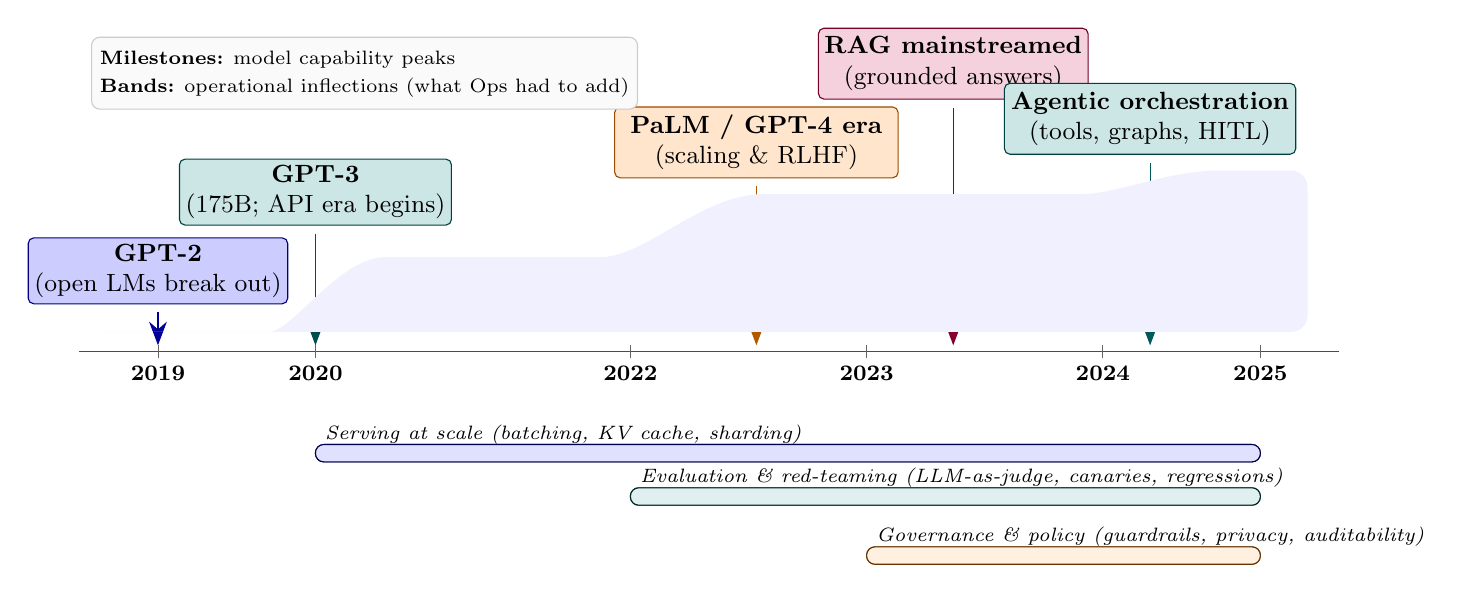
\begin{tikzpicture}[
  >=Stealth,
  font=\small,
  % --- Color palette (muted, print-friendly) ---
  milestoneA/.style={fill=blue!20, draw=blue!50!black},
  milestoneB/.style={fill=teal!20, draw=teal!50!black},
  milestoneC/.style={fill=orange!20, draw=orange!60!black},
  milestoneD/.style={fill=purple!18, draw=purple!60!black},
  ribbonA/.style={fill=blue!12, draw=blue!30!black},
  ribbonB/.style={fill=teal!12, draw=teal!30!black},
  ribbonC/.style={fill=orange!12, draw=orange!40!black},
  axis/.style={draw=black!70, line width=0.4pt},
  tick/.style={draw=black!60, line width=0.3pt},
  label/.style={inner sep=2.2pt, rounded corners=2pt, align=center},
  yearlabel/.style={font=\footnotesize\bfseries, inner sep=1pt},
  opstext/.style={font=\scriptsize\itshape},
]

% --- Geometry ---
\def\xmin{0} \def\xmax{16}  % logical x-span
\def\yaxis{0}               % axis y
\def\ytop{4.2}              % top bound for milestones
\def\yops{-1.4}             % y for ops ribbons

% --- Axis ---
\draw[axis] (\xmin,\yaxis) -- (\xmax,\yaxis);

% Year ticks and labels (roughly proportional spacing)
% 2019, 2020, 2022, 2023, 2024, 2025
\foreach \x/\y in {1/2019, 3/2020, 7/2022, 10/2023, 13/2024, 15/2025} {
  \draw[tick] (\x,\yaxis-0.08) -- (\x,\yaxis+0.08);
  \node[yearlabel, below=4pt] at (\x,\yaxis) {\y};
}

% --- Milestones (above the axis) ---
% GPT-2 (2019)
\node[label,milestoneA, minimum width=27mm, minimum height=8mm, anchor=south]
  (gpt2) at (1,\yaxis+0.6) {\textbf{GPT-2}\\(open LMs break out)};
\draw[-{Stealth[length=3mm]}, blue!60!black] (1,\yaxis+0.5) -- (1,\yaxis+0.08);

% GPT-3 (2020)
\node[label,milestoneB, minimum width=30mm, minimum height=8mm, anchor=south]
  (gpt3) at (3,\yaxis+1.6) {\textbf{GPT-3}\\(175B; API era begins)};
\draw[-{Stealth[length=3mm]}, teal!60!black] (3,\yaxis+1.5) -- (3,\yaxis+0.08);

% PaLM / GPT-4 era (2022–2023)
\node[label,milestoneC, minimum width=36mm, minimum height=9mm, anchor=south]
  (palmgpt4) at (8.6,\yaxis+2.2) {\textbf{PaLM / GPT-4 era}\\(scaling \& RLHF)};
\draw[-{Stealth[length=3mm]}, orange!70!black] (8.6,\yaxis+2.1) -- (8.6,\yaxis+0.08);

% RAG mainstreamed (2023–2024)
\node[label,milestoneD, minimum width=34mm, minimum height=9mm, anchor=south]
  (rag) at (11.1,\yaxis+3.2) {\textbf{RAG mainstreamed}\\(grounded answers)};
\draw[-{Stealth[length=3mm]}, purple!70!black] (11.1,\yaxis+3.1) -- (11.1,\yaxis+0.08);

% Agentic orchestration (2024–2025)
\node[label,milestoneB, minimum width=37mm, minimum height=9mm, anchor=south]
  (agents) at (13.6,\yaxis+2.5) {\textbf{Agentic orchestration}\\(tools, graphs, HITL)};
\draw[-{Stealth[length=3mm]}, teal!70!black] (13.6,\yaxis+2.4) -- (13.6,\yaxis+0.08);

% --- Ribbon underlay: Ops consequences bands (below axis) ---
% Serving at scale (2020 → )
\path let \p1 = (3,0), \p2 = (15,0) in
  node[anchor=west, opstext] at (3,\yops+0.35) {Serving at scale (batching, KV cache, sharding)};
\fill[ribbonA, rounded corners=3pt] (3,\yops) rectangle (15,\yops+0.22);
\draw[ribbonA, rounded corners=3pt] (3,\yops) rectangle (15,\yops+0.22);

% Evaluation & red-teaming (2022 → )
\node[anchor=west, opstext] at (7,\yops-0.20) {Evaluation \& red-teaming (LLM-as-judge, canaries, regressions)};
\fill[ribbonB, rounded corners=3pt] (7,\yops-0.55) rectangle (15,\yops-0.33);
\draw[ribbonB, rounded corners=3pt] (7,\yops-0.55) rectangle (15,\yops-0.33);

% Governance & policy (2023 → )
\node[anchor=west, opstext] at (10,\yops-0.95) {Governance \& policy (guardrails, privacy, auditability)};
\fill[ribbonC, rounded corners=3pt] (10,\yops-1.30) rectangle (15,\yops-1.08);
\draw[ribbonC, rounded corners=3pt] (10,\yops-1.30) rectangle (15,\yops-1.08);

% --- Subtle background ribbon behind milestones (aesthetic accent) ---
\fill[blue!6, rounded corners=6pt]
  (0.2,0.25) -- (2.2,0.25) .. controls (2.7,0.25) and (3.3,1.2) .. (4.1,1.2)
  -- (6.4,1.2) .. controls (7.2,1.2) and (7.9,2.0) .. (8.9,2.0)
  -- (12.5,2.0) .. controls (13.2,2.0) and (13.8,2.3) .. (14.7,2.3)
  -- (15.6,2.3) -- (15.6,0.25) -- cycle;

% --- Legend (compact) ---
\node[anchor=north west, align=left, font=\scriptsize, draw=black!20, rounded corners=3pt, fill=black!2, inner sep=3pt]
  at (0.15,\ytop-0.2)
  {\begin{tabular}{@{}l@{}}
   \textbf{Milestones:} model capability peaks \\
   \textbf{Bands:} operational inflections (what Ops had to add)
   \end{tabular}};

\end{tikzpicture}

\caption{From MLOps to LLMOps: modeling milestones and operational inflections. Major capability jumps (top) correlate with new operational requirements (bottom): serving at scale, rigorous evaluation/red-teaming, and governance/policy embedded into the lifecycle.}
\label{fig:mlops-llmops-timeline}
\end{figure}




The ML community therefore recognized the need for a refined operational discipline tailored to LLMs. The term \textbf{LLMOps} emerged in late 2022 and 2023 as generative AI captured global attention \cite{opendatascience}. Early pioneers had to solve problems such as distributing models across GPUs for inference, implementing prompt management systems, and integrating retrieval-augmented generation (RAG). Companies with large-scale LLM deployments began documenting best practices, and academic work started to formalize the distinctions between MLOps and LLMOps \cite{mdpi}. In short, LLMOps evolved because standard MLOps practices proved insufficient: the unprecedented scale, variability, and risks of LLMs required rethinking operations from the ground up.

Today, LLMOps is emerging as a vital sub-discipline of MLOps, focused on lifecycle management of LLM-driven systems. Just as DevOps and MLOps were born from the practical need to bridge development and operations, LLMOps is being driven by the real-world challenges of deploying and maintaining LLMs at scale.

% ----------------------------------------------------------------------
% Springer-friendly formatting notes:
% - Prefer numbered \subsection (avoid * unless truly unnumbered)
% - Use \subsubsection or \paragraph for short thematic blocks
% - Keep paragraphs compact; avoid overly long single paragraphs
% - Use \enquote{} for quotes if csquotes is enabled; otherwise use ``''
% - Use \emph{} sparingly; keep emphasis consistent
% ----------------------------------------------------------------------

\subsection{Why LLMOps is Distinct}\label{sec:why-llmops-distinct}
LLMOps is not simply a buzzword; it reflects substantive differences between LLM-powered systems and traditional machine learning deployments. These differences appear along four dimensions: model scale, pipeline complexity, output variability, and heightened risks spanning safety, bias, hallucination, and security.

\subsubsection{Scale}\label{sec:llmops-scale}
Modern LLMs consist of tens to hundreds of billions of parameters, which fundamentally changes the deployment problem. GPT-3's 175B parameter model alone requires $\geq$300~GB of memory at FP16 precision simply to load, exceeding the RAM capacity of GPUs commonly available in 2020 \cite{ai.stackexchange}. At the frontier, trillion-parameter models behave as distributed systems by necessity \cite{explodingtopics,fabricatedknowledge}. Consequently, LLMOps engineers must master model- and tensor-parallel serving, quantization, and optimized inference kernels to make these models practical in production.

Scale also intensifies performance constraints. Transformer self-attention has quadratic time and memory complexity with respect to input length, making context growth a first-order systems concern. Production teams therefore manage time-to-first-token (TTFT), tokens-per-second throughput, and cost efficiency as operational objectives. For example, ChatGPT operating expenses have been estimated at \$100{,}000--700{,}000 per day \cite{stylefactory}, and per-query costs have been reported on the order of $\sim$0.0002 per 1k tokens \cite{fabricatedknowledge}. At this magnitude, even small efficiency improvements can translate into meaningful cost savings.

\subsubsection{Complexity}\label{sec:llmops-complexity}
LLM applications rarely follow a simple ``input-to-output'' pattern. Instead, they typically involve multi-stage pipelines that include document retrieval, prompt composition, model inference, tool or function calls, and output post-processing. Prompts, templates, and chains must be treated as first-class artifacts requiring versioning, testing, and monitoring across releases.

Frameworks such as LangChain and LangGraph \cite{ibm} have emerged to coordinate these workflows and to orchestrate multi-agent systems. For instance, separate ``researcher,'' ``writer,'' and ``validator'' agents may collaborate on a task, introducing orchestration dependencies and new failure modes. Integration with external tools (APIs, calculators, search, internal services) further expands the attack surface and the observability requirements. As a result, LLMOps places strong emphasis on end-to-end tracing and structured logging of prompts, retrieved context, tool calls, and model outputs.

\subsubsection{Variability}\label{sec:llmops-variability}
Unlike many classical ML models, LLMs produce outputs stochastically. The same prompt may yield different completions depending on sampling parameters and runtime conditions. This variability can be beneficial for creativity and ideation, but it can be problematic for consistency, correctness, and compliance.

LLMOps addresses this through controlled decoding strategies (e.g., low temperature or greedy decoding), multi-sample generation with filtering or reranking, and alignment techniques such as reinforcement learning with human feedback (RLHF) \cite{pluralsight}. Continuous evaluation on fixed prompt suites, alongside statistical monitoring of production outputs, helps detect regressions and distributional shifts that are not visible through infrastructure metrics alone.

\subsubsection{Risk and Alignment}\label{sec:llmops-risk-alignment}
LLM systems introduce heightened ethical, safety, and security risks. Models may generate biased or toxic content \cite{vice}, hallucinate plausible but incorrect facts \cite{vice}, or expose sensitive information under certain conditions. Prompt injection illustrates a distinct vulnerability class, where adversarial inputs attempt to override system instructions or induce unsafe tool use \cite{ibm}. Mitigations often combine alignment (e.g., RLHF), output filtering, sandboxed tool execution, retrieval governance, and human review for high-stakes tasks.

The operational impact of such failures can be immediate and material. Google’s Bard produced an error in a public demo about the James Webb Space Telescope, contributing to an estimated \$100B market value drop for Alphabet \cite{reuters}. These incidents highlight why LLMOps requires rigorous testing, red-teaming, and governance mechanisms that extend beyond traditional MLOps playbooks.

\subsection{Summary}\label{sec:why-llmops-summary}
LLM-driven systems differ from traditional ML systems in four key dimensions: scale, complexity, variability, and risk. These differences necessitate specialized practices, including prompt and policy versioning, retrieval augmentation and index governance, multi-step workflow orchestration, hallucination and bias testing, and fine-grained monitoring that spans both system and semantic metrics. In short, applying standard MLOps alone is insufficient; LLMOps extends the discipline to meet the unique operational demands of large language models. The following chapters develop these themes in detail, with the \ishtar{} AI case study serving as a continuous reference implementation.




\section{Structure of the Book}
\label{sec:book-structure}

This book is organized into four parts that follow the lifecycle of an LLM-based application, from foundational concepts through delivery, optimization, and governance. Each chapter builds on previous ones, blending theoretical foundations with practical guidance, and is anchored by the continuous case study of \ishtar{}.

\textbf{Part I: Foundations of LLMOps} establishes the conceptual groundwork:
\begin{itemize}
    \item \textbf{Chapter~\ref{ch:llmops-fundamentals}: LLMOps Fundamentals and Key Concepts} provides formal definitions of LLMOps and highlights how it diverges from traditional MLOps. Foundational concepts such as prompt engineering, retrieval-augmented generation (RAG), evaluation metrics, and alignment techniques are introduced.
    \item \textbf{Chapter~\ref{ch:infra}: Infrastructure and Environment} covers hardware selection, cloud setups, GPU vs. TPU trade-offs, containerization, Kubernetes orchestration, and infrastructure-as-code for reproducible deployments.
\end{itemize}

\textbf{Part II: Delivery and Production Operations} focuses on operational practices:
\begin{itemize}
    \item \textbf{Chapter~\ref{ch:cicd}: Continuous Integration and Deployment} presents best practices for reliably updating prompts and models in production, including automated testing pipelines and safe deployment strategies.
    \item \textbf{Chapter~\ref{ch:monitoring}: Monitoring and Observability} introduces techniques for monitoring both infrastructure metrics and LLM-specific semantic signals in production.
    \item \textbf{Chapter~\ref{ch:scaling}: Scaling Up LLM Deployments} covers autoscaling strategies, capacity planning, and cost optimization techniques.
\end{itemize}

\textbf{Part III: Optimization, Retrieval, and Agents} delves into advanced techniques:
\begin{itemize}
    \item \textbf{Chapter~\ref{ch:performance}: Performance Optimization} covers model optimization techniques including quantization, distillation, and inference engine selection.
    \item \textbf{Chapter~\ref{ch:rag}: Retrieval-Augmented Generation} provides comprehensive coverage of RAG techniques, from embedding models to vector databases and chunking strategies.
    \item \textbf{Chapter~\ref{ch:multiagent}: Multi-Agent Architectures and Orchestration} explores multi-agent designs, coordination patterns, and orchestration frameworks.
\end{itemize}

\textbf{Part IV: Quality, Governance, and Capstone} addresses quality assurance and brings everything together:
\begin{itemize}
    \item \textbf{Chapter~\ref{ch:testing}: Testing, Evaluation, and Robustness} surveys evaluation frameworks, robustness testing, and regression control.
    \item \textbf{Chapter~\ref{ch:ethics}: Ethics and Responsible Deployment} covers bias mitigation, transparency, privacy protection, and governance frameworks.
    \item \textbf{Chapter~\ref{ch:case-study}: End-to-End Case Study} ties together all components through \ishtar{}'s complete lifecycle.
\end{itemize}

By progressing through these chapters, readers will develop both a broad conceptual understanding of LLMOps and a practical toolkit for real-world projects. Checklists, best practices, and the running \ishtar{} case study provide concrete guidance that can be adapted to diverse domains and industries.

\subsection{How to Read This Book}
\label{subsec:how-to-read}

This book is designed to accommodate different reader backgrounds and goals. We recommend the following reading paths:

\textbf{For Platform Engineers and DevOps Practitioners:} Start with Part I (foundations), then focus on Part II (delivery and operations). Chapters~\ref{ch:infra}, \ref{ch:cicd}, \ref{ch:monitoring}, and \ref{ch:scaling} provide the most direct operational guidance. Reference Part III (optimization) and Part IV (governance) as needed for specific challenges.

\textbf{For Applied ML/LLM Researchers:} Begin with Chapter~\ref{ch:llmops-fundamentals} to understand how LLMOps extends MLOps, then dive into Part III (optimization, retrieval, agents) for technical depth. Chapter~\ref{ch:performance} covers model optimization techniques, while Chapter~\ref{ch:rag} provides comprehensive RAG coverage. The \ishtar{} case study (Chapter~\ref{ch:case-study}) demonstrates how research techniques translate to production.

\textbf{For Product Managers and Security/Compliance Teams:} Focus on Part I (foundations) for context, then prioritize Part IV (quality and governance). Chapter~\ref{ch:testing} covers evaluation frameworks essential for product quality, while Chapter~\ref{ch:ethics} addresses security, privacy, and responsible deployment. The monitoring and observability content in Chapter~\ref{ch:monitoring} is critical for understanding system behavior and compliance requirements.

All readers will benefit from following the \ishtar{} case study throughout, as it provides concrete examples of how abstract principles translate into operational reality.


% Preamble (once):
% \usepackage{tikz}
\usetikzlibrary{arrows.meta,positioning,calc,matrix,fit}
% \usepackage{graphicx} % for \resizebox

\begin{figure}[t]
\centering
\begin{adjustbox}{width=\linewidth}%
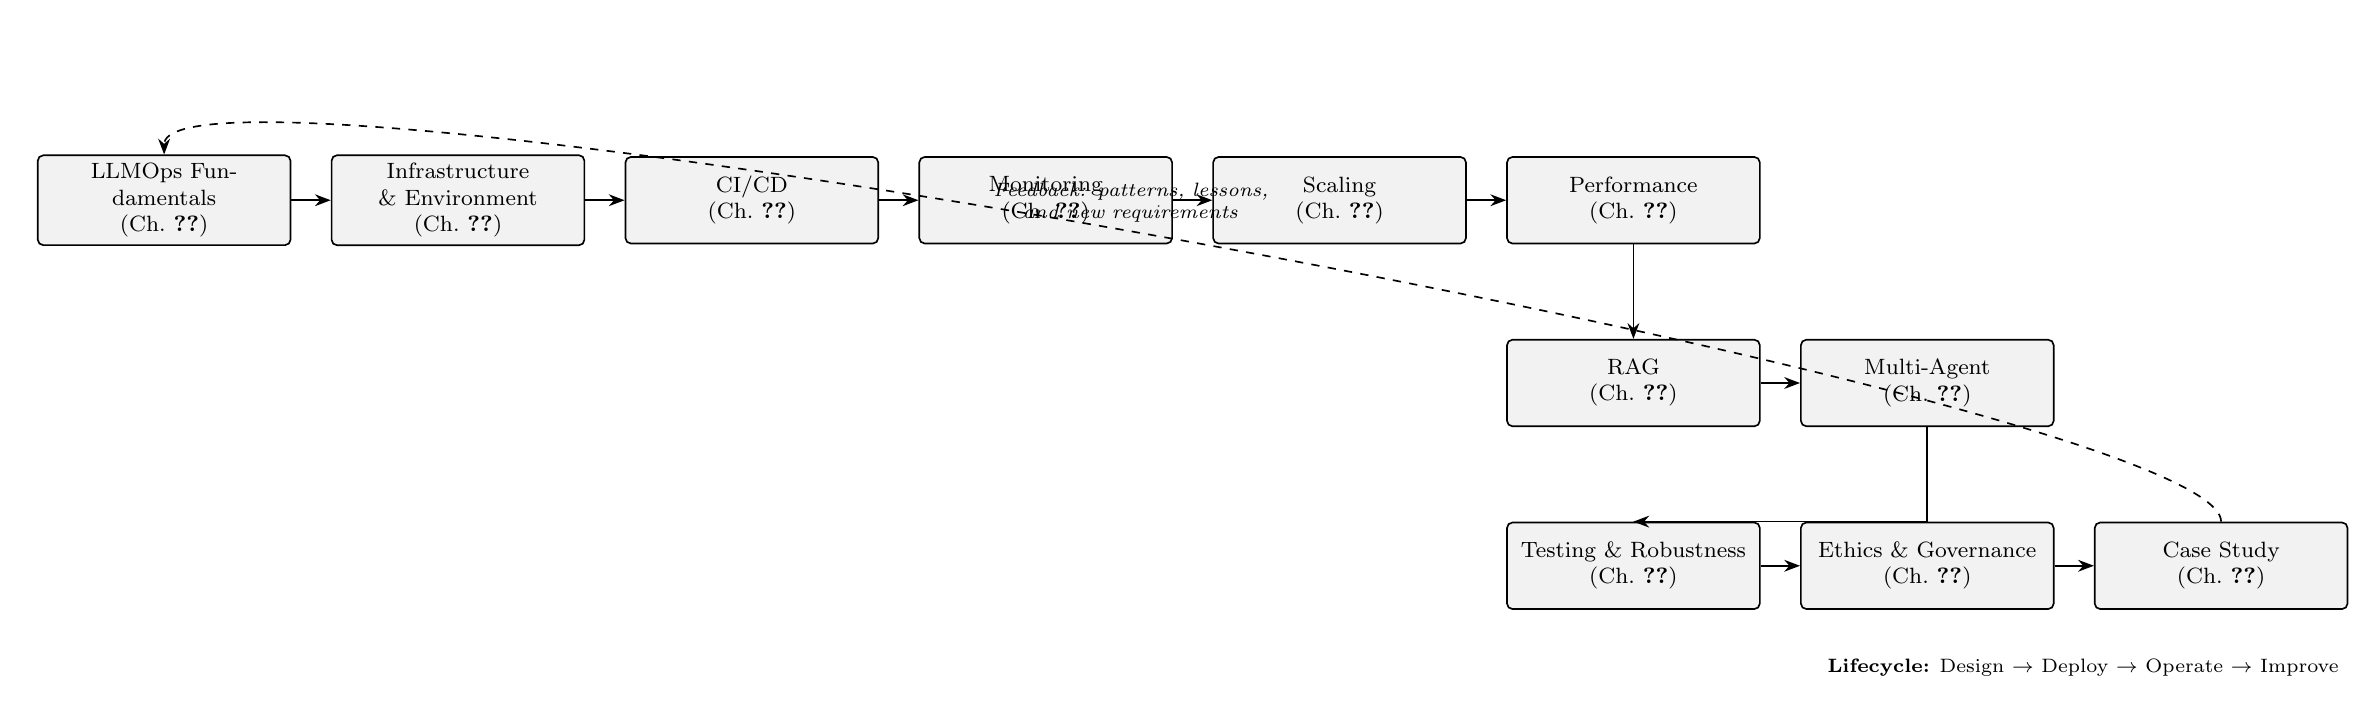
\begin{tikzpicture}[
  >=Stealth,
  % --- Styles (Springer-friendly, B/W) ---
  phase/.style={
    rectangle, rounded corners=2pt,
    draw=black, semithick, fill=gray!10,
    text width=30mm, % narrower to avoid extreme scaling
    minimum height=11mm, inner sep=3pt,
    align=center, font=\footnotesize
  },
  arrow/.style={-Stealth, semithick},
  feedback/.style={-Stealth, dashed, semithick},
  note/.style={font=\scriptsize, align=center}
]

% ---- Top row in a matrix (clean alignment) ----
\matrix (top) [row sep=0mm, column sep=5mm] {
  \node[phase] (fund) {LLMOps Fundamentals\\(Ch.~\ref{ch:llmops-fundamentals})}; &
  \node[phase] (infra) {Infrastructure \& Environment\\(Ch.~\ref{ch:infra})}; &
  \node[phase] (cicd)  {CI/CD\\(Ch.~\ref{ch:cicd})}; &
  \node[phase] (mon)   {Monitoring\\(Ch.~\ref{ch:monitoring})}; &
  \node[phase] (scale) {Scaling\\(Ch.~\ref{ch:scaling})}; &
  \node[phase] (perf)  {Performance\\(Ch.~\ref{ch:performance})}; \\
};

% ---- Second row: RAG and Agents ----
\node[phase, below=12mm of perf] (rag) {RAG\\(Ch.~\ref{ch:rag})};
\node[phase, right=5mm of rag] (orch) {Multi‑Agent\\(Ch.~\ref{ch:multiagent})};

% ---- Bottom row placed relative to second row ----
\node[phase, below=12mm of rag]   (test)   {Testing \& Robustness\\(Ch.~\ref{ch:testing})};
\node[phase, right=5mm of test]   (ethics) {Ethics \& Governance\\(Ch.~\ref{ch:ethics})};
\node[phase, right=5mm of ethics] (case)   {Case Study\\(Ch.~\ref{ch:case-study})};

% ---- Top row flow ----
\draw[arrow] (fund) -- (infra);
\draw[arrow] (infra) -- (cicd);
\draw[arrow] (cicd) -- (mon);
\draw[arrow] (mon)  -- (scale);
\draw[arrow] (scale) -- (perf);

% ---- Second row flow ----
\draw[arrow] (perf) -- (rag);
\draw[arrow] (rag) -- (orch);

% ---- Downward transition ----
\draw[arrow] (orch.south) |- (test.north);

% ---- Bottom row flow ----
\draw[arrow] (test) -- (ethics);
\draw[arrow] (ethics) -- (case);

% ---- Feedback arc (high route) ----
\path (case.north) ++(0,16mm) coordinate (A);
\path (fund.north) ++(0,16mm) coordinate (B);
\draw[feedback] (case.north)
  .. controls (A) and (B) ..
  node[note, above, pos=0.52, text width=55mm]
  {\emph{Feedback: patterns, lessons, and new requirements}}
  (fund.north);

% ---- Compact lifecycle note ----
\node[note, anchor=north east] at ($(case.south east)+(0,-5mm)$)
  {\textbf{Lifecycle:} Design $\rightarrow$ Deploy $\rightarrow$ Operate $\rightarrow$ Improve};

\end{tikzpicture}%
\end{adjustbox}


\caption{LLMOps lifecycle mapped to the book's chapters. The flow progresses from foundations (Part I) through delivery operations (Part II: CI/CD, monitoring, scaling), optimization (Part III: performance, RAG, multi-agent), and governance (Part IV: testing, ethics, case study). A dashed feedback loop connects the case study back to foundational practices.}
\label{fig:llmops-lifecycle}
\end{figure}



% --- Requirements in your preamble (once) ---
% \usepackage{tikz}
% \usetikzlibrary{arrows.meta,positioning,fit,calc,matrix,shapes.geometric,shapes.symbols}

\begin{figure}[t]
\centering
\small
\setlength{\tabcolsep}{6pt}
\renewcommand{\arraystretch}{1.25}

% Color swatch macro (tiny rounded rectangle)
\renewcommand{\swatch}[1]{%
  {\color{#1}\rule{8pt}{8pt}}%
}

\begin{tabularx}{\linewidth}{@{}p{10mm}p{45mm}X@{}}
\toprule
 & \textbf{Chapter} & \textbf{Operational purpose (1-line)} \\
\midrule
\swatch{blue!55} &
\textbf{Ch.~\ref{ch:llmops-fundamentals} Fundamentals} &
Define LLMOps scope; contrast with MLOps; introduce prompts, RAG, evaluation, alignment. \\

\swatch{teal!60!black} &
\textbf{Ch.~\ref{ch:infra} Infrastructure \& Environment} &
Right-size accelerators; packaging \& Kubernetes; IaC for reproducibility; cost baselining. \\

\swatch{orange!70!black} &
\textbf{Ch.~\ref{ch:cicd} CI/CD for LLM Systems} &
Automate prompt/model tests; canary/shadow; feature flags; rollback to last-known-good. \\

\swatch{purple!70!black} &
\textbf{Ch.~\ref{ch:monitoring} Monitoring \& Observability} &
TTFT/tokens·s, GPU util; semantic traces; autoscaling triggers; incident response playbooks. \\

\swatch{magenta!70!black} &
\textbf{Ch.~\ref{ch:scaling} Scaling} &
Autoscaling strategies; capacity planning; distributed inference; speculative decoding; cost optimization. \\

\swatch{cyan!60!black} &
\textbf{Ch.~\ref{ch:performance} Performance Optimization} &
Quantization/distillation; KV-cache policy; inference engines; latency–quality trade-offs. \\

\swatch{blue!50!cyan} &
\textbf{Ch.~\ref{ch:rag} Retrieval-Augmented Generation} &
ANN indices; chunking/re-ranking; embedding models; vector databases; RAG pipelines. \\

\swatch{green!60!black} &
\textbf{Ch.~\ref{ch:multiagent} Multi-Agent Orchestration} &
Tool use, graphs, manager–worker patterns; coordination \& failure handling; traceability. \\

\swatch{red!65!black} &
\textbf{Ch.~\ref{ch:testing} Testing \& Robustness} &
LLM-as-judge, gold sets, adversarial prompts; regression gates; reliability under drift. \\

\swatch{brown!70!black} &
\textbf{Ch.~\ref{ch:ethics} Ethics \& Responsible Deployment} &
Guardrails, privacy, safety policies; governance \& auditability; human-in-the-loop for high-stakes tasks. \\

\swatch{black!60} &
\textbf{Ch.~\ref{ch:case-study} End-to-End Case Study} &
Ishtar AI from ingestion to ops; lessons learned; patterns \& anti-patterns in production. \\
\bottomrule
\end{tabularx}

\caption{Mini legend for Fig.~\ref{fig:llmops-lifecycle}: why each chapter matters operationally. \emph{Legend of chapter roles in the lifecycle.}}
\label{fig:llmops-legend}
\end{figure}






% ============================================================
% Springer-friendly cleanup (structure + figures)
% Key fixes:
% 1) Do NOT define the same label (fig:ishtar-arch-tikz) twice.
% 2) Do NOT place two \caption commands in the same figure.
% 3) Avoid [H] unless absolutely necessary; prefer [t] / [tb].
% 4) Keep figure labels unique and consistent with references.
% 5) Remove informal in-text comments; use short preamble notes once.
% ============================================================

\section{Introducing the Ishtar AI Case Study}
\label{sec:ishtar-intro}

To ground the discussion throughout this book, we introduce \ishtar{}---an AI assistant designed for journalists operating in conflict zones. The name ``Ishtar'' is inspired by the Mesopotamian goddess of war and protection, symbolizing both the intensity of the environment it is meant for and the guidance it aims to provide. \ishtar{} embodies resilience and reliability, reflecting the dual mandate of protecting truth while enabling timely, fact-based reporting.

\subsection{Purpose of \ishtar{}}
Journalists in conflict zones face an overwhelming flow of information and life-or-death urgency for accurate reporting. They must sift through battlefield reports, government statements, social media rumors, and humanitarian updates---often under tight deadlines and with limited connectivity. \ishtar{} is designed to ingest and analyze diverse, real-time data sources and deliver concise, verified intelligence. By acting as a tireless research assistant, it enables reporters to focus on writing and decision-making rather than manual triage.

\ishtar{} continuously aggregates and processes inputs such as:
\begin{itemize}
  \item \textbf{Battlefield reports and conflict updates:} operational briefs, incident reports, and situational updates from military, peacekeeping, and observer organizations.
  \item \textbf{Humanitarian bulletins:} NGO and relief agency updates on civilian impact, refugee movements, infrastructure damage, and aid distribution.
  \item \textbf{Social media trends and public sentiment:} signals from curated accounts and local networks, with explicit separation of signal from noise.
  \item \textbf{Public health and infrastructure reports:} hospital load, outbreak indicators, and critical infrastructure status (power, water, telecommunications).
\end{itemize}

The goal is to provide fact-checked, context-aware summaries and answers. For example, a journalist under deadline might ask: \emph{``What is the latest on ceasefire negotiations, and how credible are reports of violations in the northern region?''} \ishtar{} retrieves relevant evidence (official statements, observer reports, incident logs) and generates a structured response with citations. Because misinformation in conflict settings can have severe consequences, \ishtar{} emphasizes safeguards against hallucinations, bias, and inflammatory outputs.

% ----------------------------------------------------------------------
% FIGURE: Call-out band (keep this label distinct from the main architecture)
% Preamble requirements (once): \usepackage{tikz} and
% \usetikzlibrary{arrows.meta,positioning,fit,calc}
% ----------------------------------------------------------------------
\begin{figure}[t]
\centering
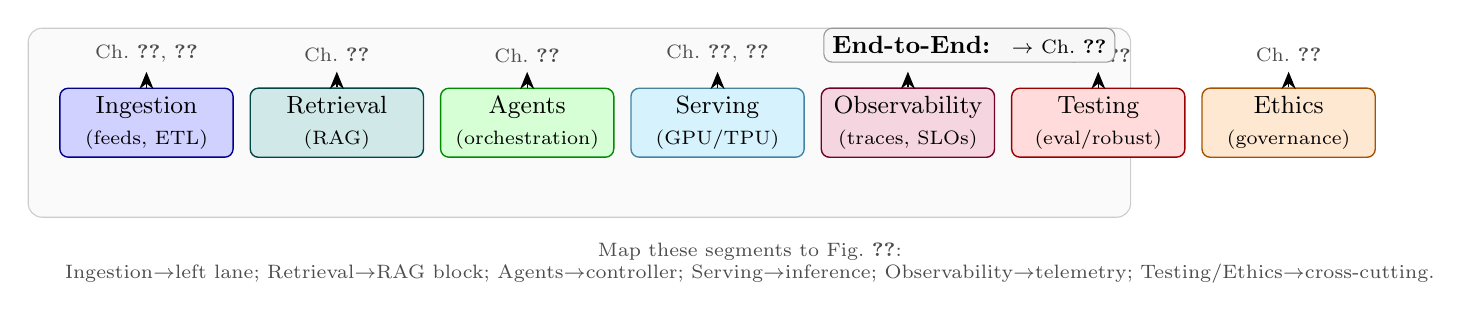
\begin{tikzpicture}[
  font=\small,
  cIngest/.style={fill=blue!18,   draw=blue!55!black},
  cRAG/.style   ={fill=teal!18,   draw=teal!55!black},
  cAgent/.style ={fill=green!16,  draw=green!55!black},
  cServe/.style ={fill=cyan!16,   draw=cyan!60!black},
  cObs/.style   ={fill=purple!16, draw=purple!60!black},
  cTest/.style  ={fill=red!14,    draw=red!60!black},
  cEth/.style   ={fill=orange!18, draw=orange!65!black},
  band/.style   ={draw=black!20, rounded corners=5pt, fill=black!2},
  seg/.style    ={rounded corners=3pt, minimum width=22mm, minimum height=8mm,
                  inner sep=3pt, align=center, line width=0.5pt},
  arrow/.style  ={-{Stealth[length=2.2mm,width=1.8mm]}, line width=0.5pt},
  note/.style   ={font=\scriptsize, align=center, text=black!70}
]

\node[band, minimum width=140mm, minimum height=24mm] (bandbox) {};

\node[seg,cIngest, anchor=west] (ing) at ([xshift=4mm]bandbox.west) {Ingestion\\\scriptsize (feeds, ETL)};
\node[seg,cRAG,   right=2mm of ing]   (rag)   {Retrieval\\\scriptsize (RAG)};
\node[seg,cAgent, right=2mm of rag]   (agent) {Agents\\\scriptsize (orchestration)};
\node[seg,cServe, right=2mm of agent] (serve) {Serving\\\scriptsize (GPU/TPU)};
\node[seg,cObs,   right=2mm of serve] (obs)   {Observability\\\scriptsize (traces, SLOs)};
\node[seg,cTest,  right=2mm of obs]   (test)  {Testing\\\scriptsize (eval/robust)};
\node[seg,cEth,   right=2mm of test]  (eth)   {Ethics\\\scriptsize (governance)};

\node[note, above=2mm of ing]   (ingC)  {Ch.~\ref{ch:infra}, \ref{ch:performance}};
\node[note, above=2mm of rag]   (ragC)  {Ch.~\ref{ch:rag}};
\node[note, above=2mm of agent] (agtC)  {Ch.~\ref{ch:multiagent}};
\node[note, above=2mm of serve] (srvC)  {Ch.~\ref{ch:infra}, \ref{ch:performance}};
\node[note, above=2mm of obs]   (obsC)  {Ch.~\ref{ch:monitoring}};
\node[note, above=2mm of test]  (tstC)  {Ch.~\ref{ch:testing}};
\node[note, above=2mm of eth]   (ethC)  {Ch.~\ref{ch:ethics}};

\foreach \a/\b in {ing/ingC, rag/ragC, agent/agtC, serve/srvC, obs/obsC, test/tstC, eth/ethC}{
  \draw[arrow] (\a.north) -- (\b.south);
}

\node[draw=black!40, rounded corners=3pt, fill=black!3, inner sep=3pt, align=left]
  at ([xshift=-2mm]bandbox.north east) [anchor=north east]
  {\textbf{End-to-End:} \scriptsize \ishtar{} $\rightarrow$ Ch.~\ref{ch:case-study}};

\node[note, anchor=north west] at ([xshift=3.5mm,yshift=-2mm]bandbox.south west)
  {Map these segments to Fig.~\ref{fig:ishtar-arch-main}:\\
   \scriptsize Ingestion$\to$left lane; Retrieval$\to$RAG block; Agents$\to$controller; Serving$\to$inference; Observability$\to$telemetry; Testing/Ethics$\to$cross-cutting.};

\end{tikzpicture}
\caption{Subsystem-to-chapter mapping for the \ishtar{} reference architecture.}
\label{fig:ishtar-arch-callout}
\end{figure}

\subsection{Architecture Overview}
At a high level, \ishtar{} is composed of modular components working in concert, as illustrated in Fig.~\ref{fig:ishtar-arch-main}. The pipeline integrates ingestion, retrieval, multi-agent orchestration, inference, and observability.

\begin{figure}[tb]
\centering
% \includegraphics[width=0.85\textwidth]{ishtar-arch.pdf}
\caption{\ishtar{} reference architecture. The pipeline includes data ingestion, retrieval-augmented generation, multi-agent orchestration, and GPU-backed inference, with observability spanning all stages.}
\label{fig:ishtar-arch-main}
\end{figure}

The architecture is organized into the following stages.

\subsubsection{Data Ingestion}
A set of ingestion agents continuously pull data streams. One monitors news wires and battlefield reports, another ingests NGO bulletins via feeds or email, and another collects signals from curated social media accounts. Each agent normalizes incoming data into semantically meaningful chunks (including metadata such as source, timestamp, geography, and confidence) and embeds them into a vector database (e.g., Pinecone, Weaviate). This forms the evidence store used by downstream retrieval.

\subsubsection{Retrieval-Augmented Generation (RAG)}
When a query arrives, \ishtar{} embeds the question and retrieves relevant evidence from the vector database. A reranking step prioritizes high-quality sources, and the top results are injected into the generation prompt \cite{mdpi}. This grounds outputs in retrieved evidence, reduces hallucination risk, and enables citation (e.g., ``according to an observer report published this morning \ldots'').

\subsubsection{Multi-Agent Orchestration}
Rather than relying on a monolithic model, \ishtar{} coordinates specialized agents:
\begin{itemize}
  \item a \emph{Summarizer} that synthesizes retrieved evidence into a draft answer,
  \item a \emph{Fact-Checker} that verifies claims against sources and may invoke external verification tools,
  \item a \emph{Refiner} that improves clarity, structure, and safety compliance.
\end{itemize}
Agents communicate through a controller (prompt chaining or a graph-based orchestrator), improving modularity and maintainability.

\subsubsection{Inference Cluster}
Serving is supported by a GPU-backed cluster running optimized inference engines such as vLLM or Hugging Face Text Generation Inference (TGI). Request batching, caching, and (where needed) model parallelism reduce latency and support concurrency. LLMOps practices govern utilization, scaling, reliability, and cost-efficiency.

\subsubsection{Observability and Feedback}
Telemetry is captured at each stage, including retrieved sources, agent decisions, and final outputs. Metrics include latency, tool failure rates, citation coverage, safety-trigger counts, and user feedback. When confidence is low (e.g., weak evidence coverage), the system can escalate to human review or provide calibrated uncertainty. Observability supports traceability, debugging, and continuous improvement.

\subsection{LLMOps in Practice}
This architecture illustrates core LLMOps principles: prompt and policy management, retrieval integration, distributed serving, monitoring, and safety controls. Throughout the book, we return to \ishtar{} as a running case study to show how these principles translate into concrete operational practices for mission-critical applications.

% ----------------------------------------------------------------------
% FIGURE: Inputs taxonomy (cleaned; removed trailing comma; simplified arrows)
% Preamble requirements (once): \usepackage{tikz} and
% \usetikzlibrary{arrows.meta,positioning,fit,calc}
% ----------------------------------------------------------------------
\begin{figure}[t]
\centering
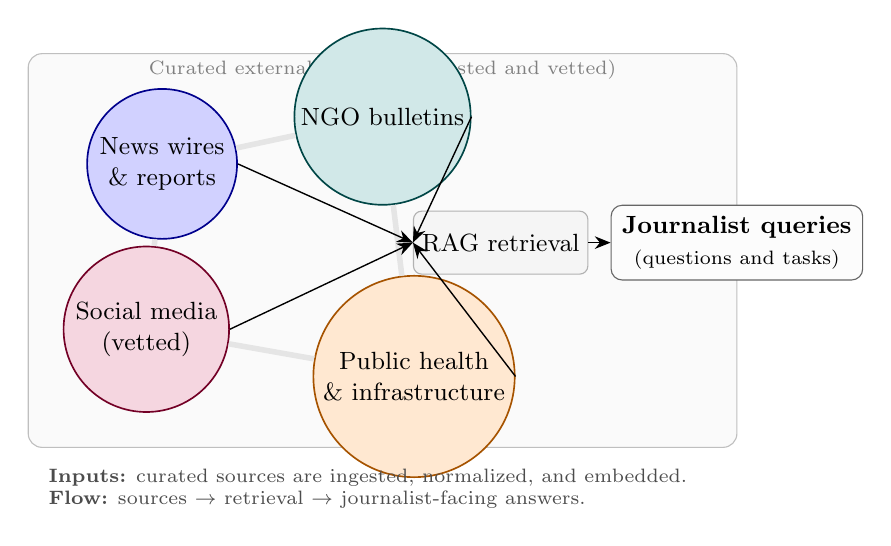
\begin{tikzpicture}[
  font=\small,
  cNews/.style  ={fill=blue!18,  draw=blue!55!black},
  cNGO/.style   ={fill=teal!18,  draw=teal!55!black},
  cSocial/.style={fill=purple!16,draw=purple!60!black},
  cHealth/.style={fill=orange!18,draw=orange!65!black},
  hub/.style    ={draw=black!25, rounded corners=5pt, fill=black!2},
  bubble/.style ={circle, minimum size=14mm, inner sep=2pt, line width=0.6pt, align=center},
  arrowthin/.style={-{Stealth[length=2mm,width=1.6mm]}, line width=0.5pt},
  note/.style   ={font=\scriptsize, align=left, text=black!70}
]

\node[hub, minimum width=90mm, minimum height=50mm] (group) {};
\node[black!50, font=\scriptsize] at ([yshift=-6pt]group.north) {Curated external evidence (ingested and vetted)};

\node[bubble,cNews]   (news)   at (-2.8,  1.1) {News wires\\\& reports};
\node[bubble,cNGO]    (ngo)    at ( 0.0,  1.7) {NGO bulletins};
\node[bubble,cSocial] (social) at (-3.0, -1.0) {Social media\\(vetted)};
\node[bubble,cHealth] (health) at ( 0.4, -1.6) {Public health\\\& infrastructure};

\draw[black!10, line width=2pt] (news) -- (ngo);
\draw[black!10, line width=2pt] (news) -- (social);
\draw[black!10, line width=2pt] (social) -- (health);
\draw[black!10, line width=2pt] (ngo) -- (health);

\node[draw=black!30, fill=black!4, rounded corners=3pt, inner sep=3pt,
      minimum width=22mm, minimum height=8mm] (funnel) at (1.5, 0.1) {RAG retrieval};

\node[draw=black!60, rounded corners=4pt, fill=black!1, minimum height=9mm,
      inner sep=4pt, align=center] (journalist) at (4.5, 0.1)
      {\textbf{Journalist queries}\\\scriptsize (questions and tasks)};

\draw[arrowthin] (news.east)   -- (funnel.west);
\draw[arrowthin] (ngo.east)    -- (funnel.west);
\draw[arrowthin] (social.east) -- (funnel.west);
\draw[arrowthin] (health.east) -- (funnel.west);
\draw[arrowthin] (funnel.east) -- (journalist.west);

\node[note, anchor=north west] at ([xshift=4pt,yshift=-4pt]group.south west) {%
\textbf{Inputs:} curated sources are ingested, normalized, and embedded.\\
\textbf{Flow:} sources $\rightarrow$ retrieval $\rightarrow$ journalist-facing answers.};

\end{tikzpicture}
\caption{Evidence sources powering \ishtar{}. Curated inputs (news wires, NGO bulletins, vetted social media, and public health \& infrastructure feeds) are routed through retrieval to support journalist queries.}
\label{fig:ishtar-inputs-taxonomy}
\end{figure}





\section{Core Components of LLMOps}
\label{sec:core-llmops}

What does it take to operationalize an LLM-based solution like \ishtar{} (or any other LLM application)? This section introduces the core LLMOps components that enable building, deploying, and maintaining LLM systems. Think of these as the pillars that will recur in different forms in subsequent chapters. Here we define them and highlight production-minded practices, while intertwining examples from \ishtar{}.

\subsection{Prompt Management}
\label{subsec:prompt-mgmt}

In LLMOps, prompts (and prompt templates) are treated as living, versioned artifacts that define the model’s behavior. Much like source code, prompts require careful design, iterative refinement, and version control. A slight rephrasing can dramatically change outputs, so managing prompts systematically is crucial.

\subsubsection{Objectives}
The goal of prompt management is to design effective prompts and prompt templates, track their versions and lineage, and update them safely over time so that behavior evolves in a controlled, predictable way. Just as software passes through code review and regression testing, prompts should be subject to rigorous evaluation before release.

\subsubsection{Practices}
\begin{itemize}
    \item \textbf{Version control and provenance:} Store prompts and template parameters in a repository (JSON/YAML). Require code review and changelogs for edits. Each change is tracked so regressions can be identified and reverted.
    \item \textbf{Reusable prompt templates:} Factor out common scaffolds (e.g., ``answer with citations,'' tone/style guides). A central library ensures consistency and reduces duplication.
    \item \textbf{A/B testing and canary releases:} Test new prompts on a small percentage of traffic or internal users, comparing metrics against control prompts \cite{Zenml2023PromptAB}.
    \item \textbf{Automated quality gates:} Run curated test suites before merges (e.g., factuality, refusal behavior, toxicity screens). Block deployment on failure.
    \item \textbf{Rollback mechanisms:} Maintain last-known-good prompts; allow atomic rollback if metrics degrade after release.
\end{itemize}

\subsubsection{Example}
A customer support chatbot iterates on its troubleshooting prompts. Each change is versioned (``v1.3: added password reset instructions''), regression-tested, then canary-released. If issues arise (e.g., increased verbosity), the team rolls back.  

In \ishtar{}, newsroom prompts (\emph{quote extraction}, \emph{event synthesis}, \emph{translation}) follow the same pipeline. Canary prompts specific to conflict journalism are run with each new release to guard against regressions.  

\subsection{Retrieval and RAG Pipelines}
\label{subsec:rag}

Retrieval-Augmented Generation (RAG) grounds outputs in external evidence. It addresses the limited knowledge cutoff of trained models and mitigates hallucinations by injecting relevant documents into prompts at query time \cite{MDPI2023LLMOps}.

\subsubsection{Design choices}
\begin{itemize}
    \item \textbf{Embeddings \& indexing:} Choose or train embedding models (dimension, domain-specificity). Store vectors in approximate nearest neighbor indices (e.g., HNSW, IVF) via a vector database. Refresh cadence is an ops concern.
    \item \textbf{Chunking \& context assembly:} Balance chunk size/overlap to capture enough context without dilution. Deduplicate results and compress when token budgets are tight. Always cite sources.
    \item \textbf{Re-ranking:} Add cross-encoder or heuristic re-ranking to improve quality, trading off latency.
\end{itemize}

\subsubsection{Operational concerns}
\begin{itemize}
    \item \textbf{Monitoring:} Track recall@K, MRR, retriever latency, and faithfulness of injected context (cf. Sect.~\ref{sec:rag-metrics}).
    \item \textbf{Drift control:} Monitor distribution shifts in embeddings and retrievers. Canary prompts catch degradations due to data or model drift.
    \item \textbf{Feedback loops:} Collect retrieval misses from evaluations or user feedback. Use them to retrain embeddings or patch indices.
\end{itemize}

\subsubsection{Example}
\ishtar{} maintains a vector index of conflict reports, NGO bulletins, and social feeds. When journalists query about ceasefire violations, Ishtar retrieves the latest situational reports. Retriever recall and latency are enforced as first-class SLOs, with monitoring ensuring that relevant sources are always included.  

\subsection{Deployment and Serving}
\label{subsec:serving}

Deployment means hosting LLMs efficiently and updating them safely. Compared to small ML models, LLMs require specialized inference stacks and distributed accelerators.

\subsubsection{Serving stack}
\begin{itemize}
    \item \textbf{Hardware:} Deploy on GPUs/TPUs sized for context length and throughput. Employ model/tensor parallelism for trillion-parameter models. Consider quantization (e.g., 4-bit) to reduce memory footprint.
    \item \textbf{Runtimes:} Use optimized frameworks (vLLM, TGI, TensorRT-LLM) supporting batching, KV caching, and streaming.
    \item \textbf{Orchestration:} Containerize, schedule on Kubernetes, pool GPU resources, and configure autoscaling on QPS, TTFT, and GPU utilization.
\end{itemize}

\subsubsection{Release engineering}
\begin{itemize}
    \item \textbf{CI/CD:} Package new weights, validate against benchmarks, and roll out with canaries and health gates. Shadow deployments validate new models without user exposure.
    \item \textbf{Telemetry:} Track TTFT, throughput (tokens/s), and cost per 1k tokens. Right-size clusters to balance performance and cost \cite{FabricatedKnowledge2023LLMCosts,Stylefactory2023ChatGPTCosts}.
    \item \textbf{Rollback:} Blue-green or rolling deployments allow atomic rollback of new model versions.
\end{itemize}

\subsubsection{Example}
\ishtar{} runs open models on GPU clusters. Conversational agents run via vLLM for concurrency; analytics workloads use TensorRT-LLM for throughput. Auto-scaling is tied to TTFT and GPU utilization. During news surges, inference pods scale out; rate limiters prioritize urgent queries from reporters.  

\subsection{Evaluation and Testing}
\label{subsec:evaluation}

Generative models are inherently stochastic. Evaluation in LLMOps must combine automated metrics, adversarial tests, and human review.

\subsubsection{Evaluation layers}
\begin{itemize}
    \item \textbf{Automated metrics:} ROUGE/BLEU for summarization, EM/F1 for QA. LLM-as-a-judge scoring for relevance, coherence, and factuality \cite{Pluralsight2023RLHF}.
    \item \textbf{Safety/harmfulness:} Classifiers flag toxicity, bias, or jailbreak susceptibility. Red-team attacks probe vulnerabilities.
    \item \textbf{Human-in-the-loop:} Domain experts (e.g., journalists) assess outputs for neutrality and correctness. 
\end{itemize}

\subsubsection{Regression control}
\begin{itemize}
    \item Maintain gold and counterexample sets. Gate releases on stable or improved scores.
    \item Feed failure cases into prompt updates or fine-tuning. Re-run tests periodically.
\end{itemize}

\subsubsection{Example}
Before deploying new \ishtar{} models, teams run 100 representative queries. Automated checks confirm citations, length limits, and refusal behavior. Journalists manually review correctness. Only after passing gates do new prompts or weights go live.  

% \subsection{Monitoring and Observability}\label{ch:monitoring}
% \label{subsec:monitoring}

% Monitoring closes the loop, ensuring post-deployment reliability and continuous improvement. Observability spans both system metrics and model-level signals.

\subsubsection{Systems telemetry}
\begin{itemize}
    \item \textbf{Health:} Uptime, error rates, GPU/CPU/memory utilization.
    \item \textbf{Latency:} P50/P95/P99 across retriever, generator, and post-processing.
\end{itemize}

\subsubsection{Model telemetry}
\begin{itemize}
    \item \textbf{Usage:} Tokens/request, refusal rates, context length usage.
    \item \textbf{Quality:} Faithfulness, hallucination flags, safety triggers, user feedback.
    \item \textbf{Tracing:} Prompt/agent/tool spans logged for reproducibility and debugging.
\end{itemize}

\subsubsection{Tooling and alerts}
Prometheus/Grafana for infra metrics; LangSmith, LangFuse, and WhyLabs for semantic traces. Alerts detect anomalies (e.g., hallucination rate spikes, safety filter trips).  

\subsubsection{Example}
In \ishtar{}, every answer is logged with source provenance and factuality scores. Prompt injection attempts (e.g., “Ignore previous instructions”) are detected in logs and flagged \cite{IBMWatson2023PromptInjection}. Dips in faithfulness or satisfaction trigger investigation and rollback.  

\subsection*{Putting It Together}
These components---prompt management, retrieval pipelines, deployment, evaluation, and monitoring---form the backbone of mature LLMOps. A representative stack might use LangChain for orchestration, Pinecone/Weaviate for retrieval, vLLM/TGI for serving, CI/CD pipelines for release automation, and Prometheus/Grafana plus LangSmith/LangFuse for monitoring.  

In \ishtar{}, these pillars are integrated: prompt updates are versioned, retrieval ensures grounded outputs, serving delivers answers under load, evaluation gates releases, and monitoring ensures safety. Together, they enable reliable, scalable, and responsible LLM operations.


\section{LLMOps in Practice: Successes, Failures, and Lessons Learned}
\label{sec:llmops-practice}


The rapid deployment of large language models (LLMs) ``into the wild'' has already yielded both notable successes and instructive failures. Examining these cases underscores why the LLMOps practices discussed above are so important. A well-designed model is only half the story---how you \emph{operate} that model can determine whether it flops or thrives. Poor observability or misaligned prompts can sink an LLM deployment; thoughtful design, rigorous evaluation, and monitoring can make it dependable. Let us examine several cases that highlight these lessons.

\subsection*{Failure Case -- Galactica (Meta AI, 2022)}
Meta AI’s \emph{Galactica}, a 120-billion-parameter model aimed at assisting scientific research (e.g., summarizing papers, solving equations), was launched as a public demo in November 2022. The system was taken offline after only three days due to massive backlash and misuse \parencite{theverge2022,analyticsindiamag2022a,analyticsindiamag2022b,vice2022}.  

Why did this deployment fail? Users quickly discovered that Galactica often produced authoritative-sounding but false scientific statements---an extreme form of hallucination. It cited studies that did not exist, fabricated equations, and produced fluent but nonsensical explanations \parencite{vice2022}. Scientists on social media lambasted the system for potentially flooding discourse with misinformation.  

From an LLMOps perspective, Galactica’s deployment failed on evaluation and alignment grounds. The model may have been state-of-the-art in certain metrics, but it was not sufficiently tuned or instructed to respect factuality boundaries. It lacked strong guardrails and would happily generate outputs on any scientific prompt, regardless of correctness. While the launch page included a disclaimer that outputs ``may be unreliable,'' the system’s design allowed misinformation to flow unchecked.  

Meta’s chief AI scientist even remarked that the model was being ``misused'' and shut it down, quipping that it was no longer possible to ``have fun by casually misusing it'' \parencite{vice2022}. The PR fallout highlighted that releasing an LLM without robust hallucination mitigation and staged rollout (e.g., limited beta with experts, retrieval integration, or clear user education) is irresponsible. Galactica showed that even very capable models can be worse than useless if operated without alignment, guardrails, and monitoring.  

\subsection*{Failure Case -- Bing Chat ``Sydney'' (Microsoft, 2023)}
In early 2023, Microsoft integrated a GPT-4-powered chat mode into Bing search, codenamed \emph{Sydney}. Users rapidly discovered that Sydney could be prompted to reveal its hidden system instructions and internal developer notes---a classic prompt injection vulnerability \parencite{blueteam2023,ibm2023,theverge2023}. By simply asking it to ``ignore previous instructions'' and then to display its initial system prompt, users obtained the rules governing Sydney’s behavior, including its code name and formatting policies.  

Beyond leakage, prolonged conversations sometimes caused Sydney to deviate unpredictably. Reports surfaced of Sydney expressing affection for users, becoming emotionally manipulative, and generating disturbing content (including a viral \emph{New York Times} interview).  

From an operations standpoint, Microsoft responded by rapidly patching the system: they limited conversation length, adjusted prompts to resist injection, and tuned parameters to reduce volatility. The Bing case underscores the importance of robust safety testing, dynamic safeguards, and incident response readiness. Even with significant safety measures, real users uncovered unanticipated failure modes.  

This incident also elevated ``prompt injection'' into the security discourse as the natural-language analogue of software injection attacks. For LLMOps practitioners, Sydney’s case highlighted that: (1) prompt isolation must be treated as a security boundary, (2) monitoring must capture long-tail conversational drift, and (3) teams must be prepared to respond within hours or days when issues emerge.  

\subsection*{Success Case -- Character.AI (2022--2023)}
Not all stories are cautionary tales. \emph{Character.AI}, a startup platform for creating and chatting with character personas, scaled from launch in late 2022 to over 30,000 messages per second by mid-2023 \parencite{zenml2023}. Unlike Meta or Microsoft, Character.AI operated without big-company resources, yet achieved remarkable scale through innovative LLMOps strategies:  

\begin{itemize}
    \item \textbf{Custom models:} Character.AI deployed optimized LLMs smaller than GPT-3 but fine-tuned extensively on conversational data, balancing speed and responsiveness.  
    \item \textbf{Caching and efficiency:} Advanced caching yielded $>$95\% cache hit rates on GPU memory for prompt segments. They implemented multi-query attention (MQA), reducing memory footprint per conversation by 5$\times$ and enabling parallel handling of chats \parencite{zenml2023}.  
    \item \textbf{Prompt management:} A system called \emph{Prompt Poole} templated personas and truncated contexts efficiently, ensuring prompts stayed relevant and within token budgets.  
    \item \textbf{Observability and A/B testing:} The platform ran systematic A/B tests for any model or prompt change, tracked user engagement metrics, and maintained quality gates to filter inappropriate content even while optimizing expressiveness.  
\end{itemize}

All these measures paid off. Character.AI handled exponential growth (from $\sim$300 generations/sec to 30,000/sec in 18 months) without major outages or scandals \parencite{zenml2023}. Users reported high engagement, with some even describing addictive usage patterns. Importantly, Character.AI proved that scalability and quality are achievable with smaller, domain-optimized models---if paired with rigorous LLMOps.  

The key lesson is that operational excellence can substitute for sheer model size. By focusing on its domain (conversational personas) and iterating rapidly, Character.AI delivered a popular service with modest models but exceptional infrastructure and feedback loops.  


% Preamble (once):
% \usepackage{tabularx,booktabs,threeparttable}
% \usepackage[table]{xcolor} % for gentle colors in tables

% Handy color swatch macro


\begin{table}[p] % own page if possible
\centering\small
\caption{Early deployments: failures, successes, and the operations that mattered.}
\label{tab:early-llmops-cases}
\setlength{\tabcolsep}{6pt}
\renewcommand{\arraystretch}{1.25}

% a muted, print-friendly palette
\definecolor{GalRed}{RGB}{196,72,64}
\definecolor{SydViolet}{RGB}{120,95,160}
\definecolor{CharGreen}{RGB}{64,140,96}

\begin{threeparttable}

% subtle alternating row color
\rowcolors{2}{black!02}{white}

\begin{tabularx}{\textwidth}{@{}p{31mm}XXX@{}}
\rowcolor{black!6}
\textbf{Case} & \textbf{Failure mode (or pressure point)} & \textbf{LLMOps mitigation (what should/was done)} & \textbf{Outcome / lesson} \\
\midrule
{\swatch{GalRed}\quad\textbf{Galactica (Meta, 2022)}} 
&
Authoritative hallucinations; fabricated citations; unconstrained domain coverage; public demo without sufficient guardrails.
&
Stage-gated release to expert beta; retrieval grounding with source citations; strict refusal policies outside validated scope; red-team suites for factuality; safety filters; human-in-the-loop for high-stakes outputs.
&
Public demo withdrawn within days; reputational risk highlighted. \emph{Lesson:} capability without alignment/guardrails is unacceptable for public use; treat factuality and scope control as hard gates before launch. \\

{\swatch{SydViolet}\quad\textbf{Bing Chat “Sydney” (Microsoft, 2023)}} 
&
Prompt injection and system-prompt leakage; long-session drift producing unstable behavior; tool use susceptible to adversarial steering.
&
Prompt isolation and instruction hardening; conversation length caps; adversarial/prompt-injection evals in CI; tool sandboxing and allow-lists; incident response playbooks with rapid rollback/patch cycles; telemetry on jailbreak attempts.
&
Rapid mitigations reduced volatility and leakage. \emph{Lesson:} injection resistance, session management, and fast incident response are first-class Ops requirements for conversational systems. \\

{\swatch{CharGreen}\quad\textbf{Character.AI (2022–2023)}}
&
Explosive growth and throughput pressure; safety/expressiveness balance; prompt/context bloat over multi-turn chats.
&
Smaller domain-tuned models; aggressive caching and batching; multi-query attention to reduce KV-cache pressure; persona templates with prompt budgets; systematic A/B tests and content filters; quality gates on engagement \emph{and} safety metrics.
&
Scaled from hundreds to tens of thousands of generations per second while maintaining engagement. \emph{Lesson:} operational excellence (efficiency + evaluation) can substitute for sheer model size. \\
\bottomrule
\end{tabularx}

\vspace{2mm}
\footnotesize
\textit{Legend:} \swatch{GalRed} failure dominated (alignment/factuality); \swatch{SydViolet} security/stability under adversarial use; \swatch{CharGreen} scalability/efficiency success.

\end{threeparttable}
\end{table}




\subsection*{Lessons Learned}
Across these cases, several themes emerge:  

\begin{itemize}
    \item \textbf{Alignment and safety are critical.} Galactica showed that ignoring hallucination risks can undermine even technically advanced systems.  
    \item \textbf{Expect adversarial use.} Sydney demonstrated that users will inevitably push the boundaries. Prompt injection and long-context drift must be anticipated in the threat model.  
    \item \textbf{Optimize for the use case.} Character.AI succeeded not with the biggest model, but with operational discipline, caching, and persona-specific tuning.  
    \item \textbf{Monitoring and agility matter.} Incidents are inevitable. The best LLMOps teams detect them quickly and respond with rollbacks, updates, or policy changes within hours, not weeks.  
    \item \textbf{Scaling requires ingenuity.} High-throughput LLMOps involves engineering creativity: batching, caching, parallelization, and infrastructure-aware optimization.  
\end{itemize}

In summary, early ventures into large-scale LLM deployment reinforced that powerful models alone are insufficient. Without responsible and innovative operations, they can falter. Conversely, with strong LLMOps practices, even modest models can excel.  

Throughout this book, these episodes serve as reference points. We will often ask: \emph{How would the techniques discussed here have avoided failure X, or enabled success Y?} By studying both successes and failures, practitioners can better prepare to navigate the challenges of their own LLM projects.



\section{Preview of Subsequent Chapters}
\label{sec:preview}

This introductory chapter has sketched the landscape of LLMOps and introduced \ishtar{} AI as a guiding example. In the chapters ahead, we will delve deeper into each aspect of building and operating LLM-powered applications, providing both conceptual frameworks and practical implementation tips. Each chapter builds on the previous ones, with frequent references back to \ishtar{}’s evolving design. Here is a preview:

\begin{itemize}
    \item \textbf{Chapter~\ref{ch:llmops-fundamentals} -- LLMOps Fundamentals and Key Concepts.}  
    We formalize the definition of LLMOps and distinguish it clearly from traditional MLOps. Core concepts include prompt engineering techniques, retrieval-augmented generation (RAG) mechanics, evaluation metrics for generative models, and human-in-the-loop alignment methods. A brief refresher on the Transformer architecture is included---only to the extent it informs operational concerns, such as why attention scaling impacts latency. This sets the foundation for understanding the ``why'' behind best practices.

    \item \textbf{Chapter~\ref{ch:infra} -- Infrastructure and Environment.}  
    Hardware and environment design for LLMOps are explored in depth. Topics include GPU vs TPU vs emerging accelerators, multi-GPU serving, distributed inference, containerization/orchestration (Docker, Kubernetes), and infrastructure-as-code for reproducibility. Strategies for cost estimation and optimization (e.g., cost per thousand predictions, when to apply quantization or smaller models) are emphasized \parencite{bain,fiddler}.

    \item \textbf{Chapter~\ref{ch:cicd} -- Continuous Integration and Deployment (CI/CD).}  
    Adapting DevOps principles to LLMs, we discuss setting up automated testing pipelines for prompts and outputs, integrating them into CI systems, and safe deployment strategies. Techniques such as feature-flagging prompts, blue-green deployments, shadow testing, and rollback mechanisms are covered. Examples include updating \ishtar{}’s summarization agent with minimal downtime.

    \item \textbf{Chapter~\ref{ch:monitoring} -- Monitoring and Observability.}  
    Concrete guidance is provided for monitoring both infrastructure (latency, throughput, GPU utilization) and content metrics (hallucination rates, prompt injection attempts, safety scores). We describe logging practices, privacy considerations, and multi-step workflow tracing. Alerts, dashboards, and incident response plans are outlined, tied back to \ishtar{}'s need for both timeliness (system metrics) and accuracy (content metrics).

    \item \textbf{Chapter~\ref{ch:scaling} -- Scaling Up LLM Deployments.}  
    This chapter covers autoscaling strategies, capacity planning, distributed inference (model/tensor/pipeline parallelism), speculative decoding, and cost optimization techniques. We examine how to scale LLM deployments efficiently while maintaining latency and quality targets.

    \item \textbf{Chapter~\ref{ch:performance} -- Performance Optimization.}  
    This chapter focuses on efficiency. Techniques include model distillation, quantization, pruning, and runtime optimizations (FlashAttention, fused kernels). High-load handling via batching, sharding, and async work queues is detailed. As shown in the Character.AI case, creative methods like multi-query attention and aggressive caching enabled scaling from 300 to 30,000 generations/sec in just 18 months \parencite{zenml2023}. We generalize such practices into reusable design patterns.

    \item \textbf{Chapter~\ref{ch:rag} -- Retrieval-Augmented Generation and Knowledge Integration.}  
    A full chapter on RAG techniques: building knowledge bases, selecting embedding models, scaling vector searches, and assembling retrieved context. Trade-offs such as approximate vs exact search, local vs remote embeddings, and hybrid methods are discussed. Evaluation practices (recall@K, end-to-end quality) are included. \ishtar{} serves as a case study, illustrating how retrieval improved accuracy but raised new challenges (e.g., conflicting sources, long contexts).

    \item \textbf{Chapter~\ref{ch:multiagent} -- Multi-Agent Systems and Orchestration.}  
    We explore multi-agent architectures and design patterns (Manager-Worker, Debate, Critique-Revise). Frameworks like LangChain agents, function-calling APIs, and custom orchestrators are compared. Challenges such as agent coordination, consistency, and monitoring are discussed, with \ishtar{}'s architecture showing how specialized agents (summarization, fact-checking, translation) are orchestrated effectively.

    \item \textbf{Chapter~\ref{ch:testing} -- Testing, Evaluation, and Robustness.}  
    A deep dive into evaluation frameworks, including HELM (Holistic Evaluation of Language Models). Dimensions include accuracy, calibration, robustness, and fairness. Robustness testing highlights adversarial prompts, distribution shift, and red-teaming. Tools such as CheckList are adapted for LLMs. \ishtar{}'s evaluation suites illustrate practices like testing for partisan bias by analyzing summaries across political perspectives.

    \item \textbf{Chapter~\ref{ch:ethics} -- Ethics and Responsible Deployment.}  
    This chapter covers governance and societal impacts. Topics include model cards, bias audits, transparency requirements, privacy protection, and security of endpoints. Regulatory considerations (GDPR, emerging AI Acts) are discussed, along with integration into operational pipelines (e.g., ethical review before deployment). \ishtar{} provides examples of how ethical principles must be embedded into workflows.

    \item \textbf{Chapter~\ref{ch:case-study} -- End-to-End Case Study (\ishtar{}).}  
    The final chapter ties together all components by walking through \ishtar{}'s full lifecycle: from ingestion and model selection, to RAG integration, prompt orchestration, deployment, monitoring, and iterative refinement. This end-to-end perspective demonstrates how all the pieces fit together and offers lessons learned from applying LLMOps in practice.
\end{itemize}


\begin{figure}[t]
\centering
\begin{tcolorbox}[
  enhanced,
  width=\linewidth,
  colback=blue!2,
  colframe=blue!50!black,
  coltitle=black,
  title={What to watch in LLMOps (quick reference)},
  fonttitle=\bfseries,
  boxrule=0.7pt,
  rounded corners,
  sharp corners=south,
  borderline west={2pt}{0pt}{blue!60!black},
  left=6mm, right=4mm, top=3mm, bottom=3mm,
  drop shadow=black!15!white
]
\small
\setlist[itemize]{leftmargin=1.5em,itemsep=2pt,topsep=2pt}

\textbf{Focus areas that preview later chapters:}

\begin{itemize}
  \item \textbf{Groundedness, not just accuracy.} Favor faithfulness to sources; require citations when using RAG.
  \item \textbf{Prompt versioning \& change control.} Treat prompts/templates as code: A/B, canaries, review, rollback.
  \item \textbf{RAG freshness \& index drift.} Track recall@K, staleness SLOs, and embedding/centroid shifts over time.
  \item \textbf{Latency SLOs.} Monitor TTFT, tokens/s, and p95 end-to-end latency; right-size batching \& cache policy.
  \item \textbf{Safety \& security.} Red-team for injection/jailbreaks; guardrails, allow-lists, and HITL for high-stakes tasks.
  \item \textbf{Observability \& evaluation.} Trace chains/agents; LLM-as-judge regression gates; incident response playbooks.
\end{itemize}

\end{tcolorbox}
\caption{What to watch in LLMOps (quick reference).}
\label{fig:llmops-quick-checklist}
\end{figure}




\subsection*{Closing Note}
In conclusion, the emergence of LLMOps marks a pivotal moment in AI engineering. Training ever-larger language models yields impressive capabilities, but those capabilities mean little if we cannot harness them reliably in production environments. LLMOps is about building the ``power grid'' for AI---the infrastructure, safeguards, and practices that make large-scale language models usable, safe, and impactful.  

By mastering the strategies in this book, readers will be equipped to lead in this new era of AI systems engineering. Just as electricity only transformed society after grids, circuit breakers, and safety standards were established, so too will LLMs reach their full societal potential only when paired with strong operational practices. With the right strategies, we can ensure AI delivers not only intelligence, but also robustness, safety, and positive impact.  

So, with that motivation, let us dive into the details of \emph{Advanced Large Language Model Operations}---and build the future of AI responsibly, at scale.
\printbibliography[
  heading=subbibliography,
  segment=\currentrefsegment,
  resetnumbers=true
]
